\documentclass[11pt, oneside]{article}
\usepackage[margin=1in]{geometry}
\geometry{letterpaper}
\usepackage{graphicx}
\usepackage{amssymb}
\usepackage[parfill]{parskip}
\usepackage{amssymb}
\usepackage{amsmath}
\usepackage{listings}
\usepackage{color}
\usepackage{standalone}
\usepackage{gensymb}
\usepackage{tikz}
\usetikzlibrary{matrix,chains,positioning,decorations.pathreplacing,arrows}
\usepackage{wrapfig}
\usepackage{epstopdf}
\usepackage{float}

\graphicspath{ {code/images/} }

\def\layersep{2.5cm}

\sloppy
\definecolor{lightgray}{gray}{0.5}
\setlength{\parindent}{0pt}
\definecolor{dkgreen}{rgb}{0,0.6,0}
\definecolor{gray}{rgb}{0.5,0.5,0.5}
\definecolor{mauve}{rgb}{0.58,0,0.82}

\lstset{frame=tb,
  language=Matlab,
  aboveskip=3mm,
  belowskip=3mm,
  showstringspaces=false,
  columns=flexible,
  basicstyle={\small\ttfamily},
  numbers=none,
  numberstyle=\tiny\color{gray},
  keywordstyle=\color{blue},
  commentstyle=\color{dkgreen},
  stringstyle=\color{mauve},
  breaklines=true,
  breakatwhitespace=true,
  tabsize=3
}

\title{Neuro 120 Homework 4: Short and Long Term Memory}
\author{William Schmitt and Will Drew}
\date{Due: Thursday 15 November 2018}

\begin{document}
\maketitle

\section{Short Term Memory}

\subsection{RNN Dynamics with No Recurrent Connections}

\begin{figure}[ht!]
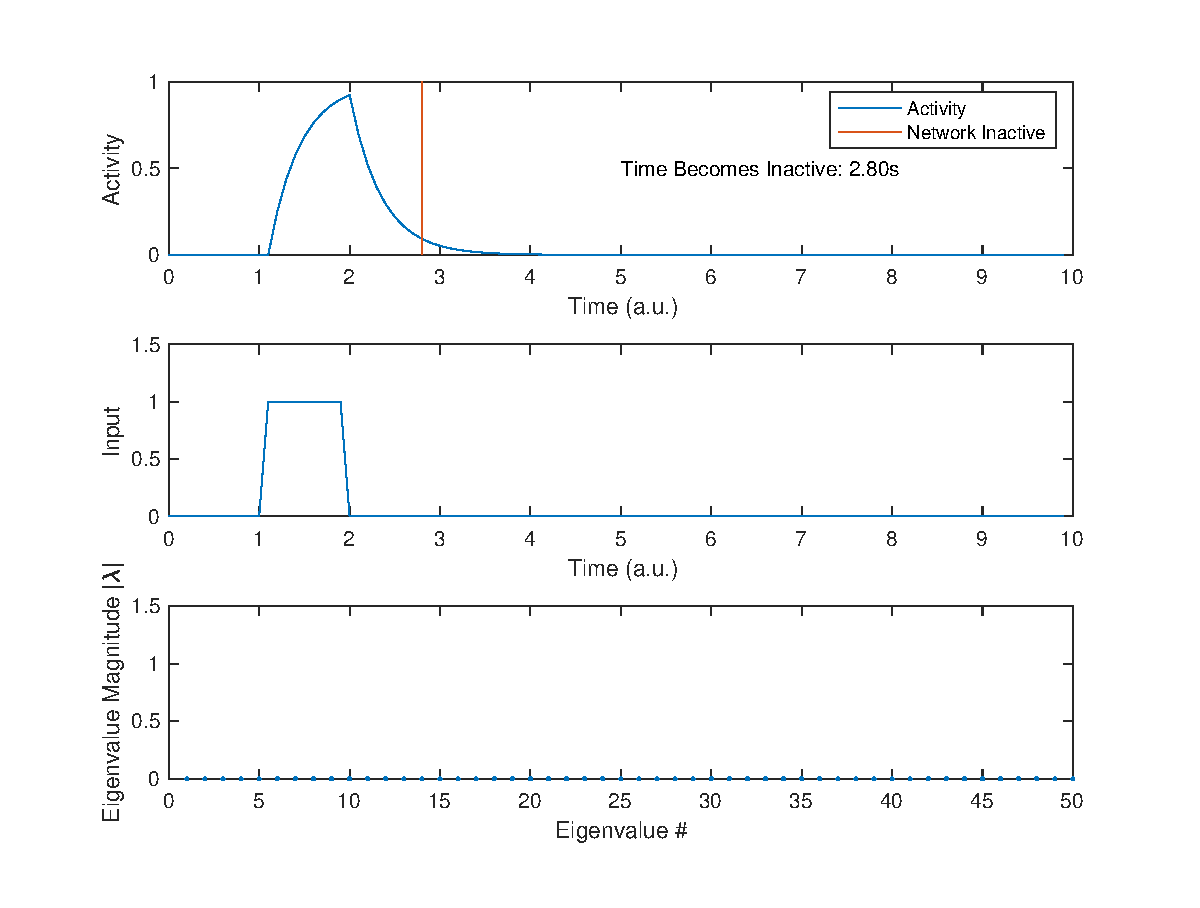
\includegraphics[width=1\textwidth]{RNNnoR.eps}
\caption{The dynamics of a RNN with no recurrent connections.}
\label{fig:RNNnoR}
\end{figure}

We build the RNN with the following code:
\lstinputlisting{code/shortterm_mem.m}
This code produces Figure \ref{fig:RNNnoR}, which we can see tells us that the activity in the network has died out at $t = 2.8$s.

\subsection{RNN with Autapses}

We comment out line 16 and uncomment line 18 and 19 of the code attached above to run the network as a set of autapses. Further, we run this three times, altering the weight scale in line 18 to be 0.9, 1, and 1.1. This produces Figures \ref{fig:RNN09}, \ref{fig:RNN10}, and \ref{fig:RNN11}.

In Figure \ref{fig:RNN09}, we see that activity in the network has not died out completely 9 seconds after the pulse, but it seems like if we expanded the time scale, the network activity would die out at around 12-14 seconds. \\
In Figure \ref{fig:RNN10}, we see that activity in the network remains stable after $t = 2$s.\\
In Figure \ref{fig:RNN11}, we see that activity in the network appears to diverge towards $+\infty$.

\begin{figure}[H]
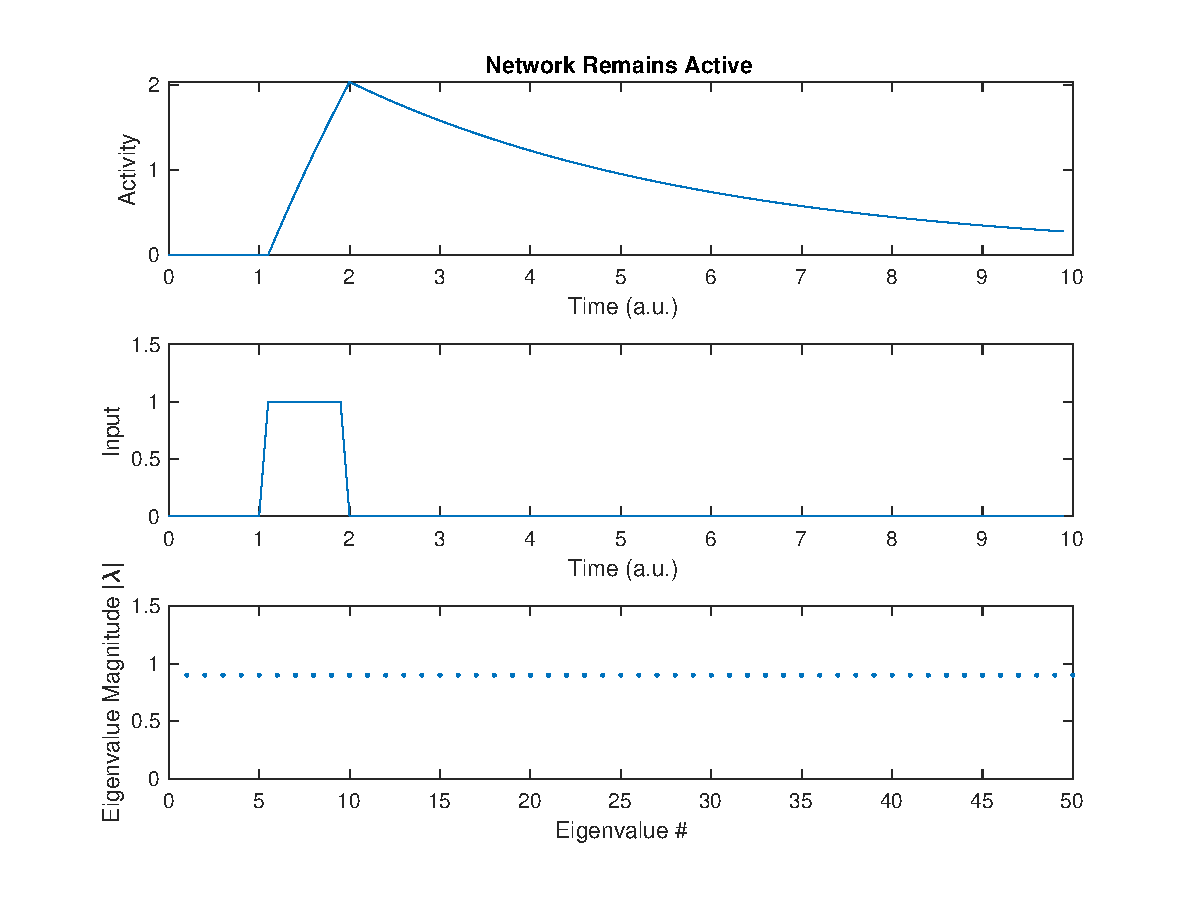
\includegraphics[width=1\textwidth]{RNN09.eps}
\caption{The dynamics of a RNN with autapses. $c = 0.9$}
\label{fig:RNN09}
\end{figure}

\begin{figure}[H]
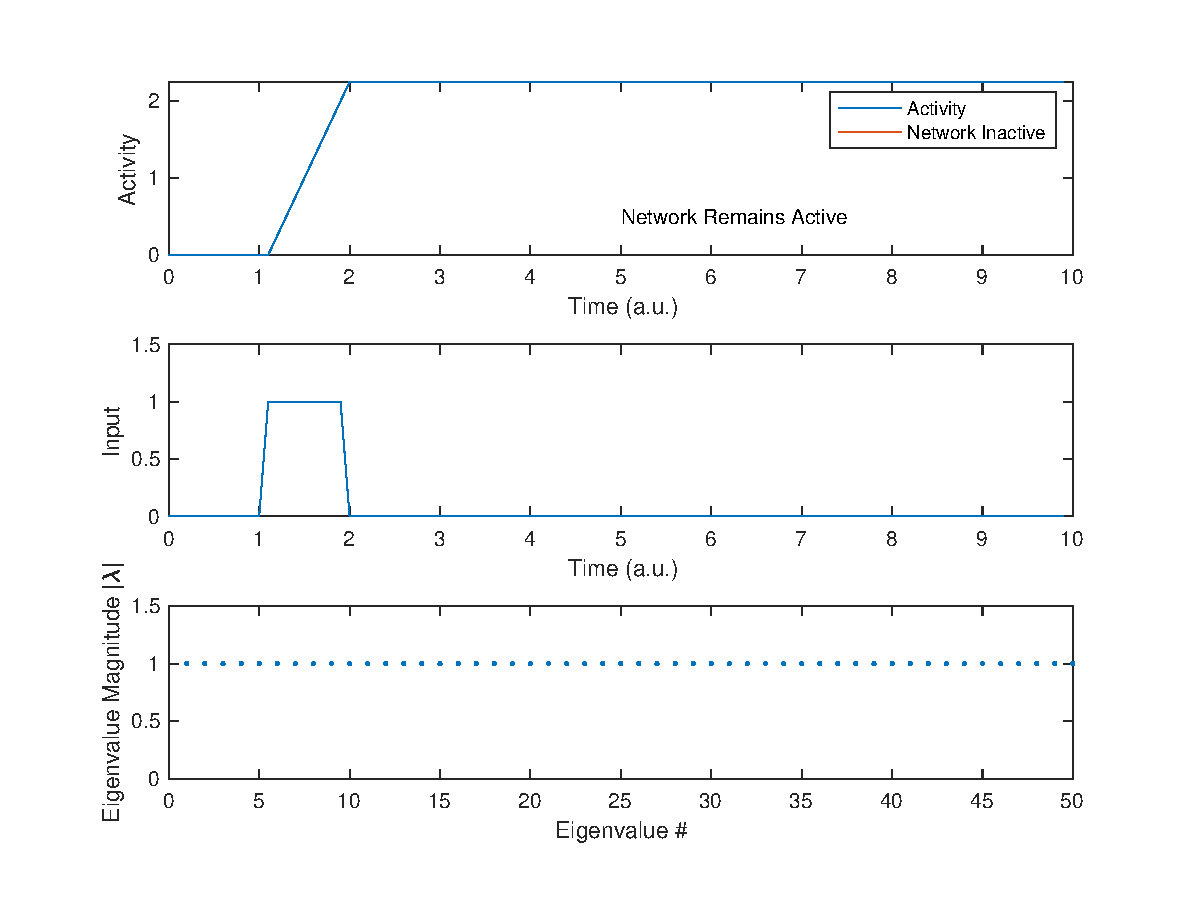
\includegraphics[width=1\textwidth]{RNN10.eps}
\caption{The dynamics of a RNN with autapses. $c = 1.0$}
\label{fig:RNN10}
\end{figure}

\begin{figure}[H]
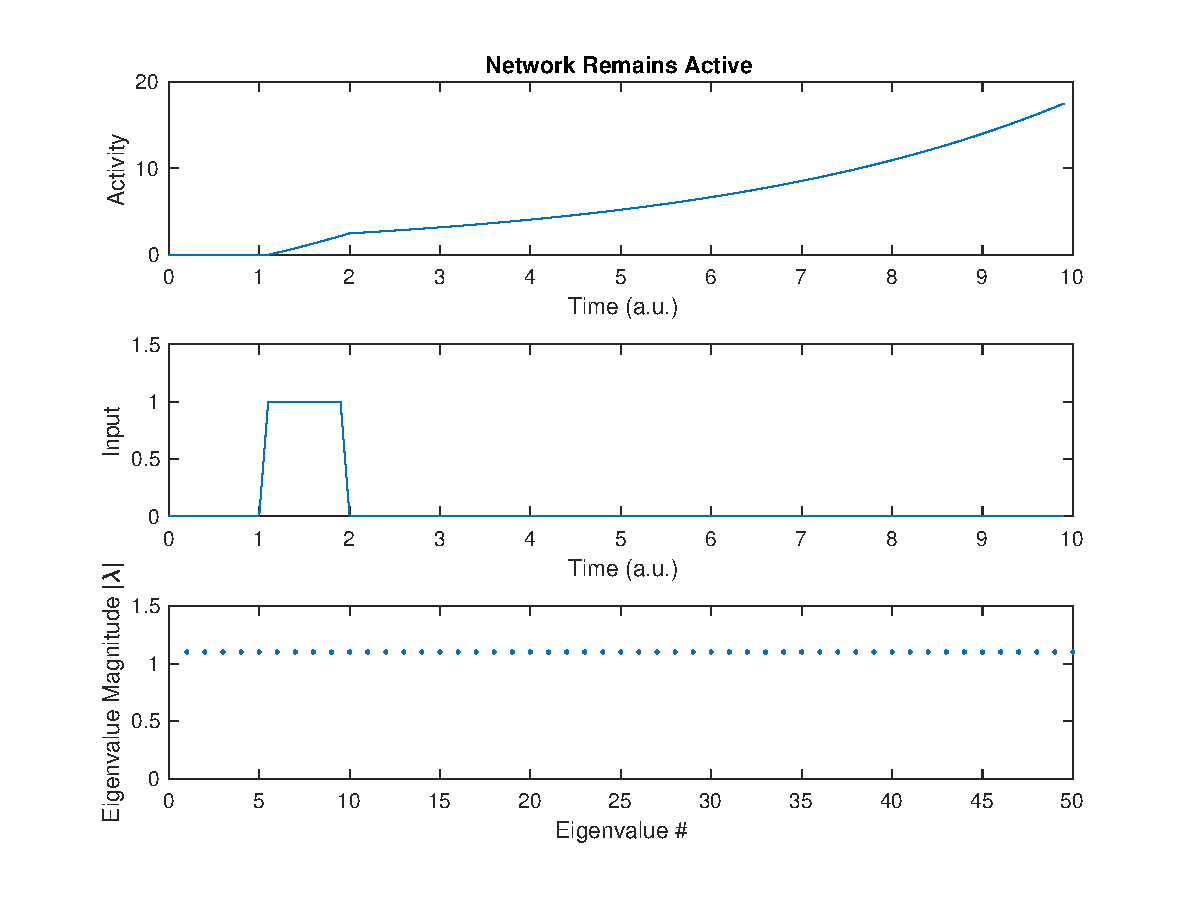
\includegraphics[width=1\textwidth]{RNN11.eps}
\caption{The dynamics of a RNN with autapses. $c = 1.1$}
\label{fig:RNN11}
\end{figure}

The magnitude of the eigenvalues of the recurrent matrix $W$ appear to be correlated with the weight scale $c$. In fact, they appear to have equal values!

We see that when the input is on, the activity increases as expected as $VI(t)$ adds to the rate of change of neuronal activity. When the input is off, that term disappears and we are left with $(c-1)r(t)$. When $c$ is less than 1 $(c=0.9)$, this term is negative, and neuronal activity decreases during this period towards 0. When $c = 1$, we see that this term is 0, indicating that there is no change in neuronal activity during this period. When $c$ is greater than 1 $(c=1.1)$, then this term is positive, indicating that neuronal activity should be increasing during this period.

Thus, the best choice of $c$ to stably store a memory would be $c=1$, as neuronal activity remains constant, neither dying out over time nor diverging towards infinity (brains crashing!).

\subsection{RNN with Interconnections}

We comment out line 19 and uncomment line 21 and 22 of the code attached above to run the network with random interconnections between neurons. Further, we run this three times, altering the weight scale in line 18 to be 0.9, 1, and 1.1. This produces Figures \ref{fig:RNN09rand}, \ref{fig:RNN10rand}, and \ref{fig:RNN11rand}.

In Figure \ref{fig:RNN09rand}, we see that activity in the network begins to calm around $t=10$s. \\
In Figure \ref{fig:RNN10rand}, we see that activity in the network does not appear to die out.\\
In Figure \ref{fig:RNN11rand}, we see that activity in the network appears to diverge towards $-\infty/+\infty$.

\begin{figure}[H]
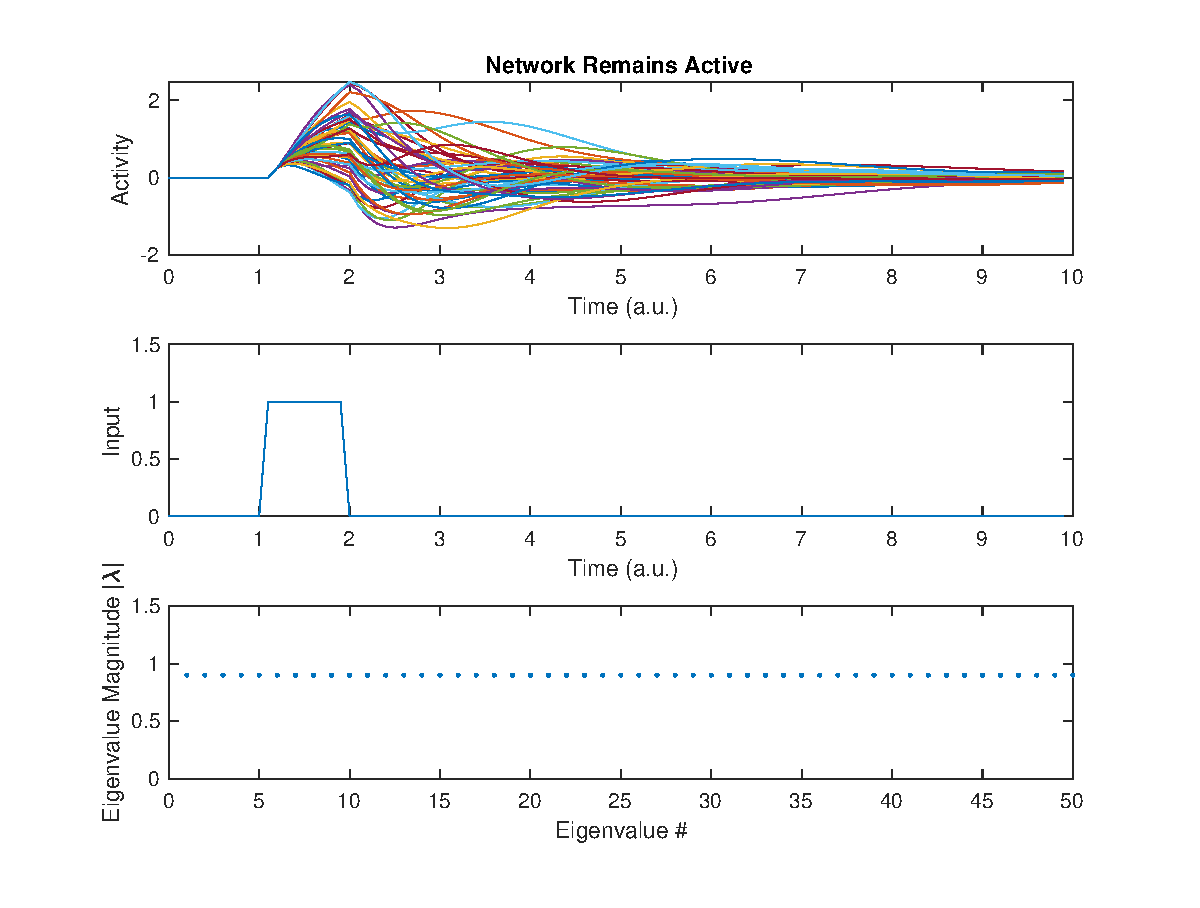
\includegraphics[width=1\textwidth]{RNN09rand.eps}
\caption{The dynamics of a RNN with interconnections. $c = 0.9$}
\label{fig:RNN09rand}
\end{figure}

\begin{figure}[H]
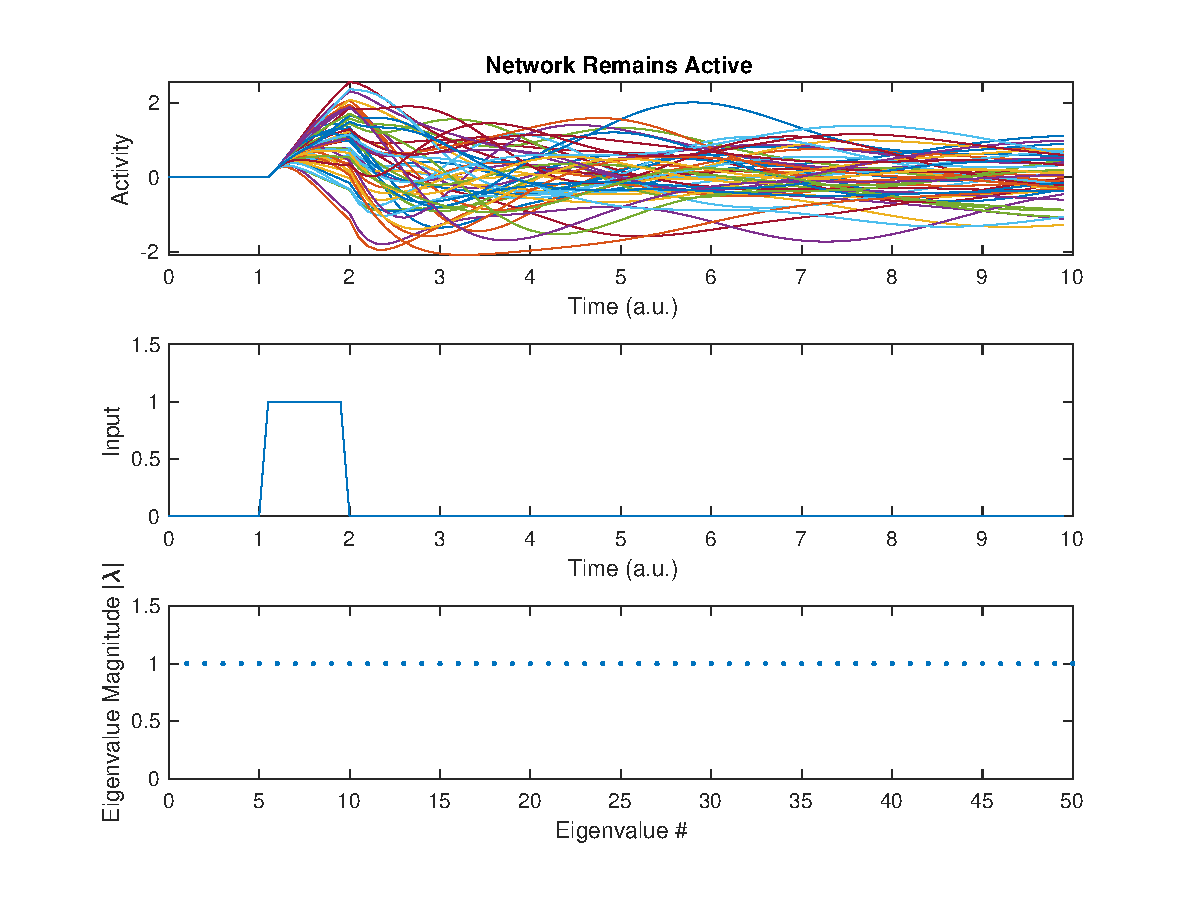
\includegraphics[width=1\textwidth]{RNN10rand.eps}
\caption{The dynamics of a RNN with interconnections. $c = 1.0$}
\label{fig:RNN10rand}
\end{figure}

\begin{figure}[H]
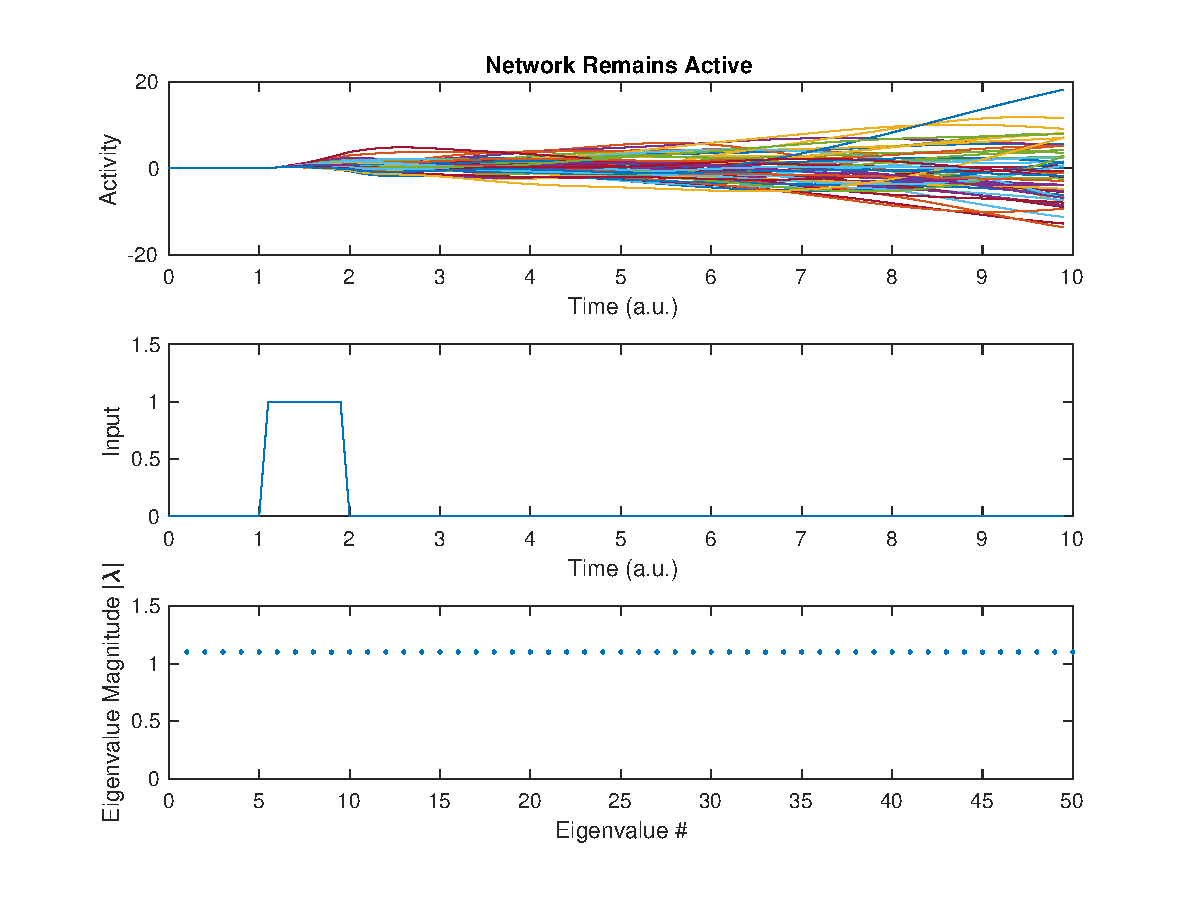
\includegraphics[width=1\textwidth]{RNN11rand.eps}
\caption{The dynamics of a RNN with interconnections. $c = 1.1$}
\label{fig:RNN11rand}
\end{figure}

The memory behavior appears to be qualitatively similar to part (b). For $c=1$, the activities in the network appear to never stop changing. Again, the magnitude of the eigenvalues of the recurrent matrix $W$ appear to be equal to the weight scale $c$. The eigenvalue magnitudes do continue to explain the memory properties of the network.

\subsection{RNN with Random Noise}

We uncomment line 24 and 25 of the code attached above to run the network with random interconnections between neurons and with random noise. Further, we run this two times, altering the weight scale in line 18 to be 0.9 and 1.0. This produces Figures \ref{fig:RNN09randnoise} and \ref{fig:RNN10randnoise}.

In Figure \ref{fig:RNN09randnoise}, we see that activity in the network begins to calm around $t=10$s. \\
In Figure \ref{fig:RNN10randnoise}, we see that activity in the network does not appear to die out.\\

\begin{figure}[H]
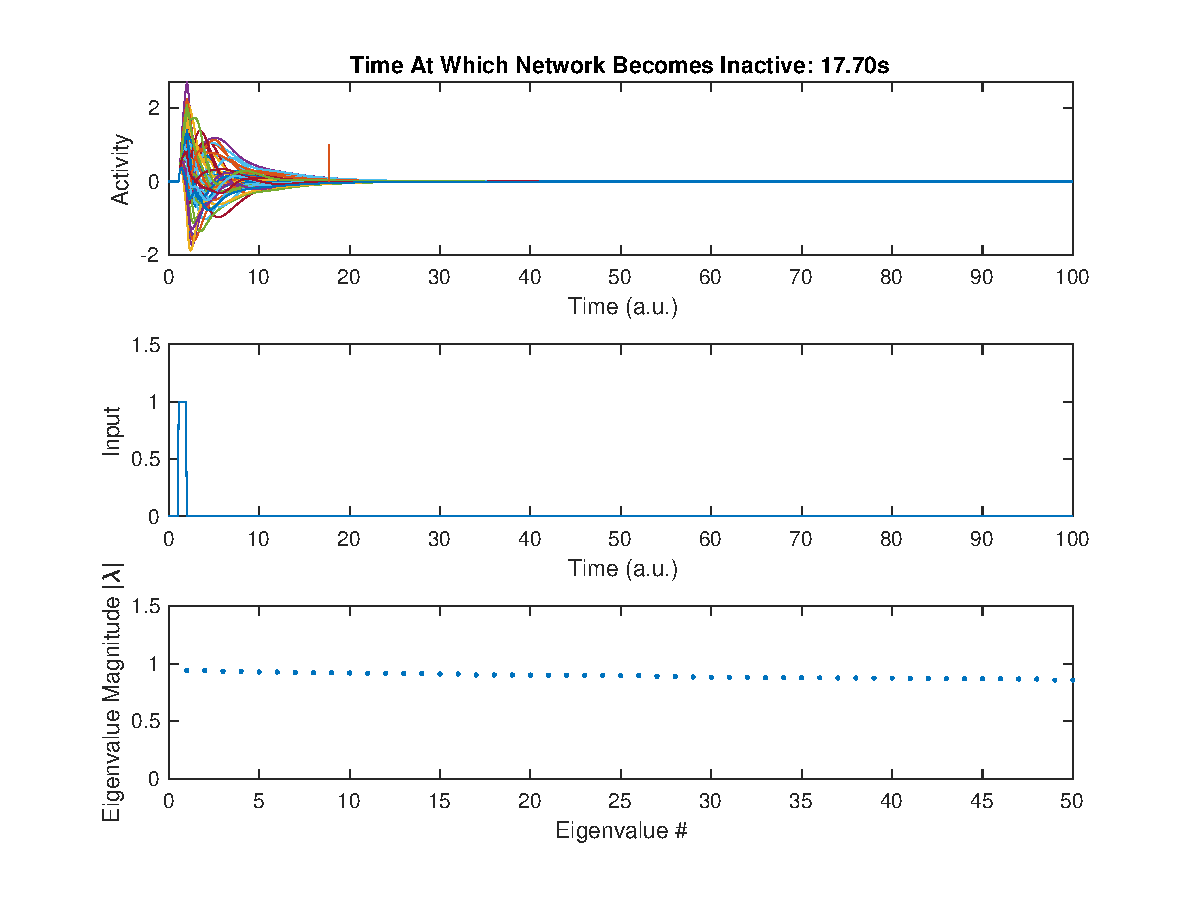
\includegraphics[width=1\textwidth]{RNN09randnoise.eps}
\caption{The dynamics of a RNN with random noise. $c = 0.9$}
\label{fig:RNN09randnoise}
\end{figure}

\begin{figure}[H]
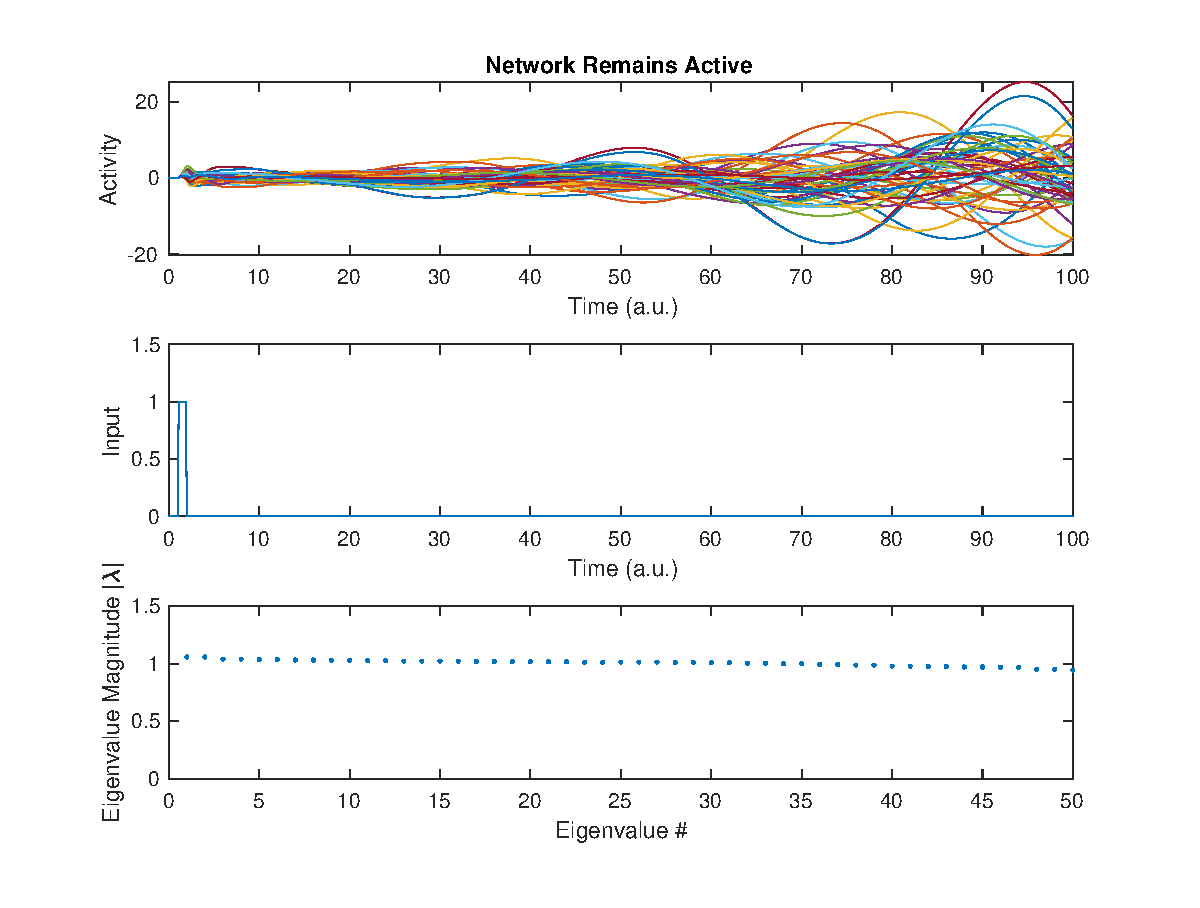
\includegraphics[width=1\textwidth]{RNN10randnoise.eps}
\caption{The dynamics of a RNN with random noise. $c = 1.0$}
\label{fig:RNN10randnoise}
\end{figure}

For $c=0.9$, the small amount of noise does not appear to significantly affect the stability of the memories. However, for $c=1$, the small amount of noise appears to destabilize the memories, with some activities even oscillating at magnitudes diverging to infinity. Looking at the eigenvalue magnitudes of the perturbed matrices, for $c=0.9$, the eigenvalue magnitudes appear to be decreasing, always less than 1. However, for $c=1.0$, the eigenvalue magnitudes start above 1, but then decrease below 1 as time goes on.

In practice, it appears that a memory with $c = 0.9$ would be better where noise is inevitable.

\section{Long Term Memory}

\begin{enumerate}
  \item Out of the 7 questions stored, it gets 6 correct.

  \item The dynamics for questions 3, 5, and 7 are shown in Figures \ref{fig:q3detail}, \ref{fig:q5detail}, and \ref{fig:q7detail}.

  For question 3, it starts off correctly constructing the appropriate answer, but then degenerates into remembering an entirely different question/answer pair.

  For question 5, it eventually reaches the correct answer for the question in about 3 steps.

  For question 7, it eventually reaches the correct answer for the question in about 3 steps.

  \item Question 3 was answered incorrectly. As seen in Figure \ref{fig:q3answer}, the network required 3 characters before the correct answer was recalled.

  \item We see the dynamics of questions 6 and 7 at varying levels of corruption in Figures \ref{fig:q6corrupt} and \ref{fig:q7corrupt}.

  The networks fails to recall question 6 at approximately 40\% and fails to recall question 7 at approximately 10\%. This means that question 6 is more strongly memorized by the network. For question 6, at 40\% corruption, we cannot make out what the correct answer is from the corrupted input, but for question 7, at 10\%, the corrupted input is still vaguely readable, enabling us to recall the correct answer.

  \item The advantages of location addressable memory is that memories can be randomly accessed and arbitrarily recalled given a target location. However, to access the memories, we must maintain an index for all memories. This is a disadvantage. Another disadvantage of location addressable memory is that if the location is lost, it is virtually impossible to retrieve the memory, even if you remember a part of it.

  The advantages and disadvantages of content addressable memories are nearly the opposite of those for location adressable memories. Addressable memories can be retrieved by partial memories and do not require indexing. However, recalled memories can be confabulated as a partial memory can be mistaken as a reference to an entirely different one. In general, content addressable memory recall is not 100\% reliable, as other memory errors can also occur.

  Content addressable memories might be better when trying to recall memories that may not be very clear, but location addressable memories ensure perfect recall if indexing is complete.


\end{enumerate}

 \begin{figure}[H]
  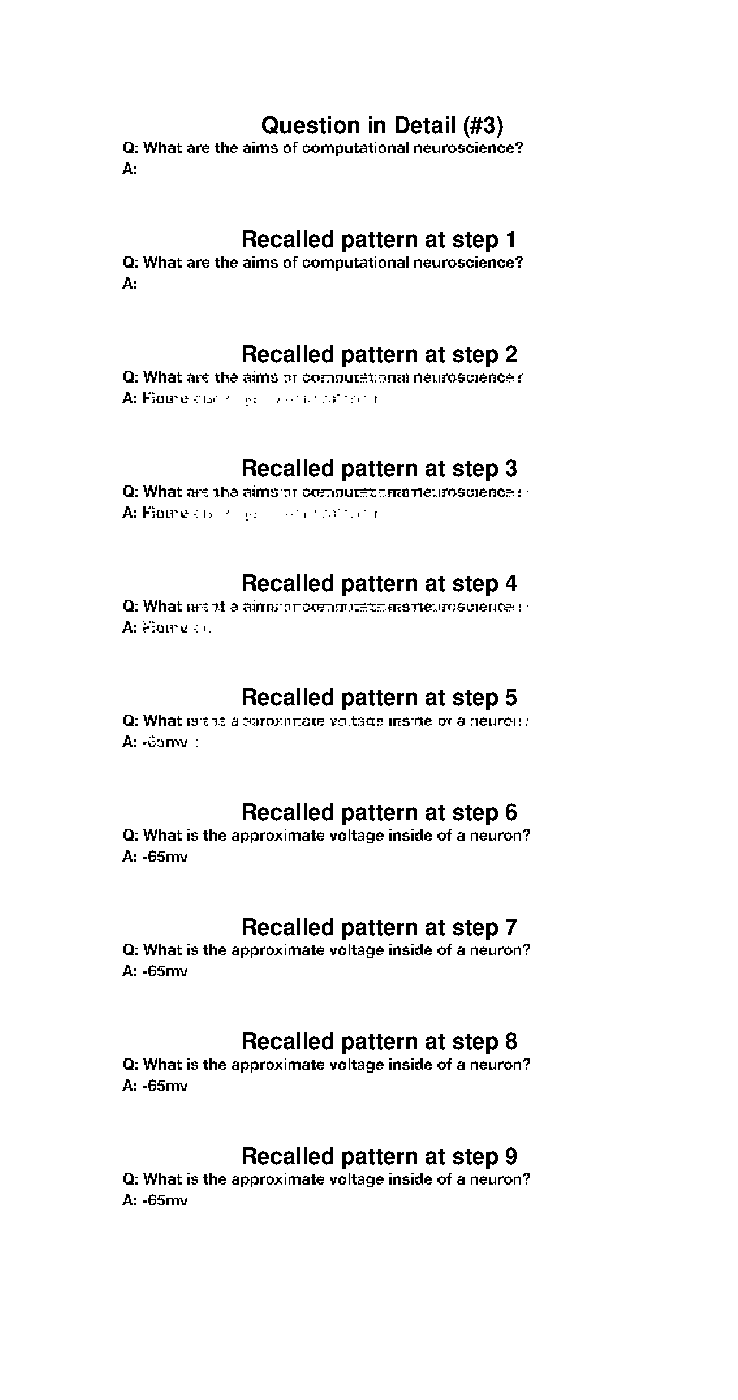
\includegraphics[width=1\textwidth]{q3detail.eps}
  \caption{The dynamics for question 3.}
  \label{fig:q3detail}
  \end{figure}

  \begin{figure}[H]
  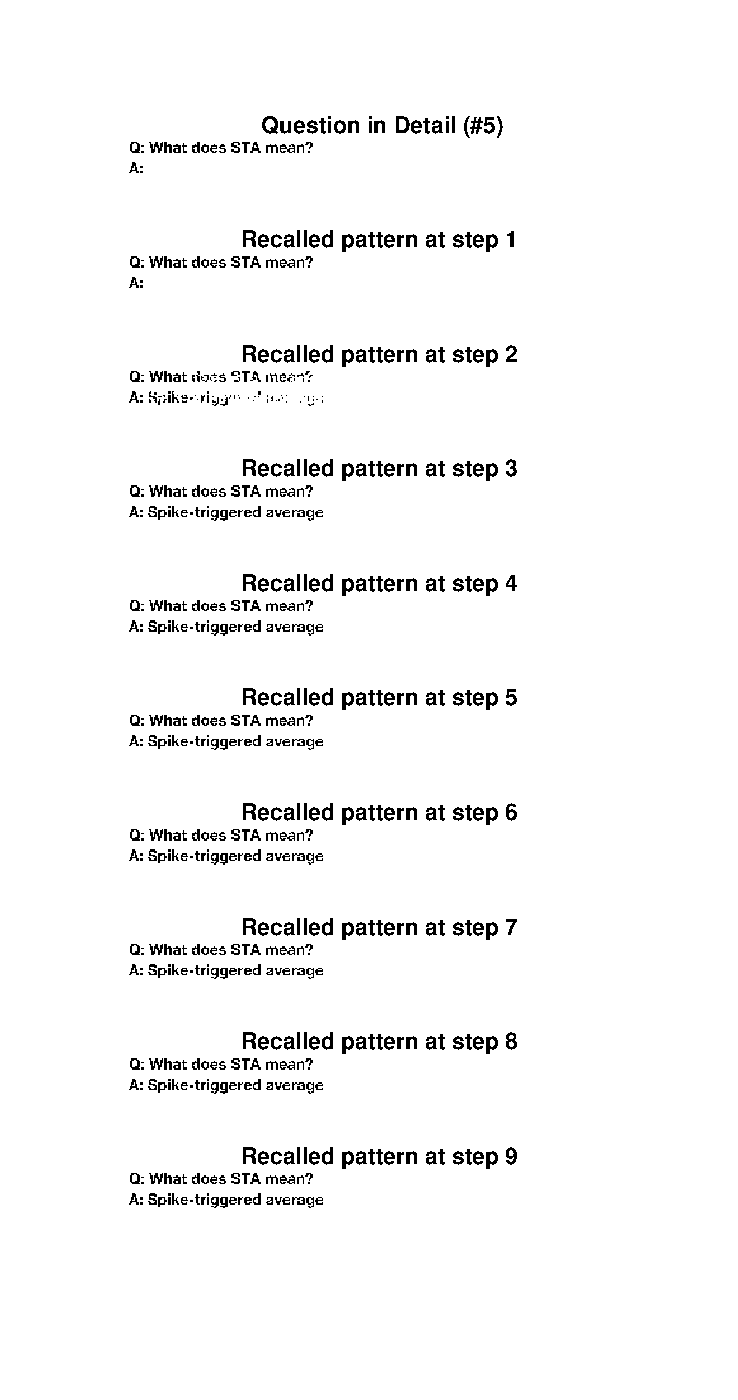
\includegraphics[width=1\textwidth]{q5detail.eps}
  \caption{The dynamics for question 5.}
  \label{fig:q5detail}
  \end{figure}

  \begin{figure}[H]
  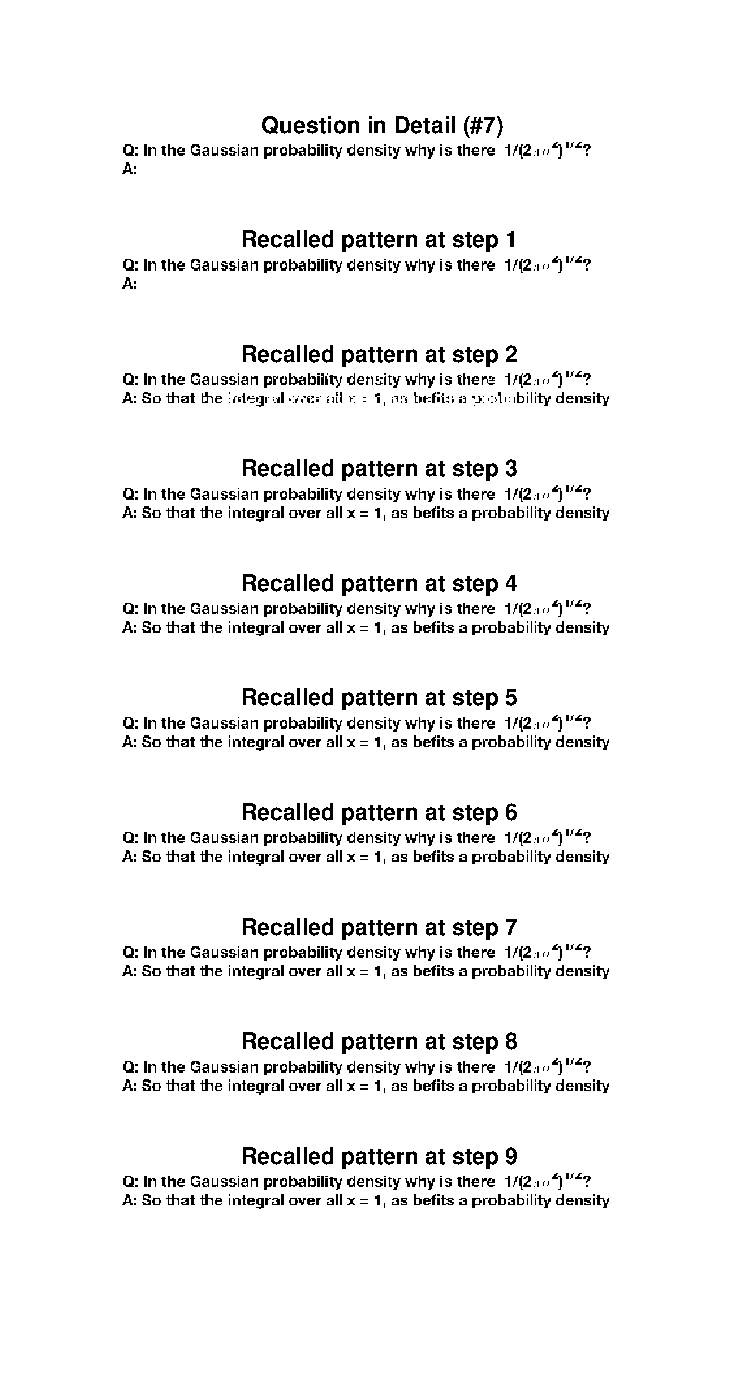
\includegraphics[width=1\textwidth]{q7detail.eps}
  \caption{The dynamics for question 7.}
  \label{fig:q7detail}
  \end{figure}

  \begin{figure}[H]
  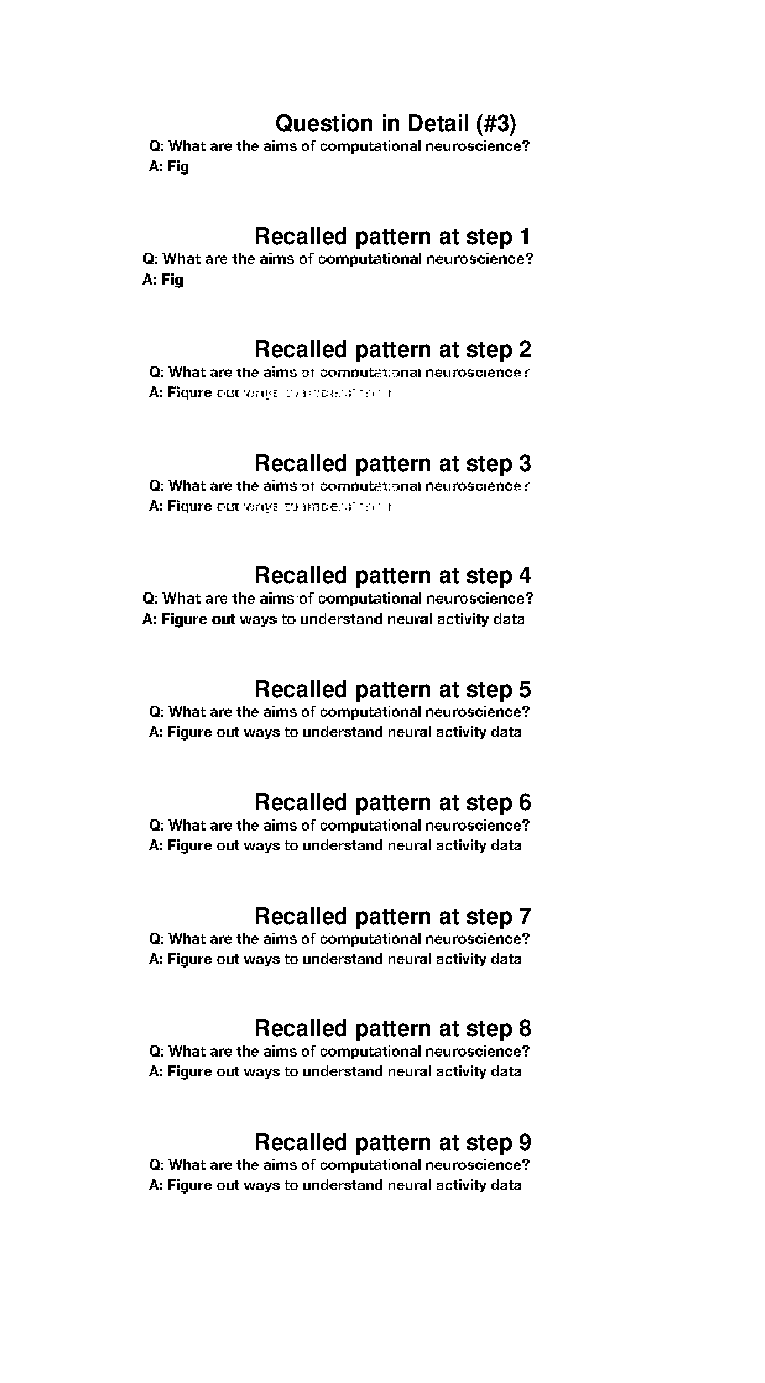
\includegraphics[width=1\textwidth]{q3answer.eps}
  \caption{The dynamics for question 3 given 3 starting characters for the answer.}
  \label{fig:q3answer}
  \end{figure}

  \begin{figure}[H]
  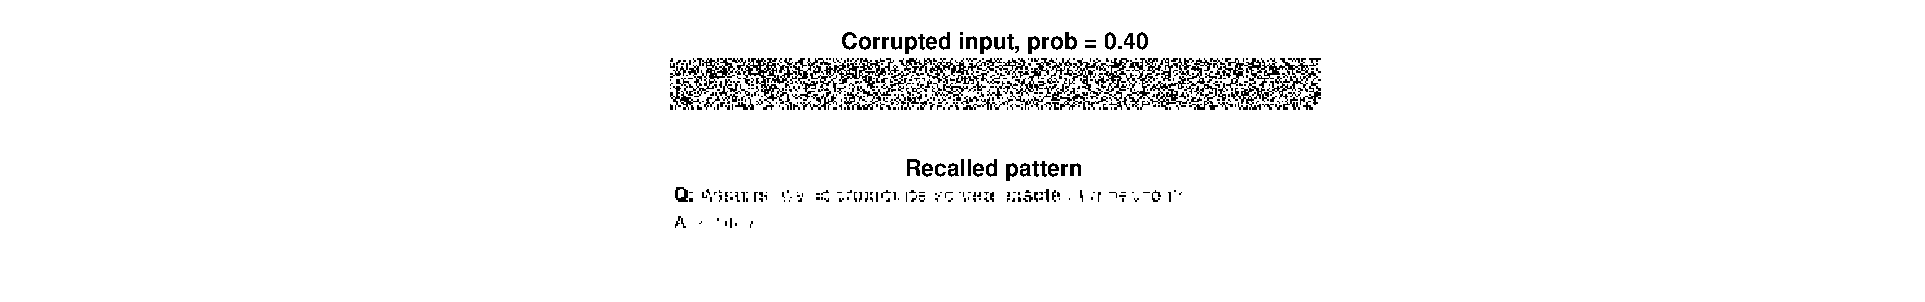
\includegraphics[width=1\textwidth]{q6corrupt.eps}
  \caption{The dynamics for question 6 at different levels of corruption.}
  \label{fig:q6corrupt}
  \end{figure}

  \begin{figure}[H]
  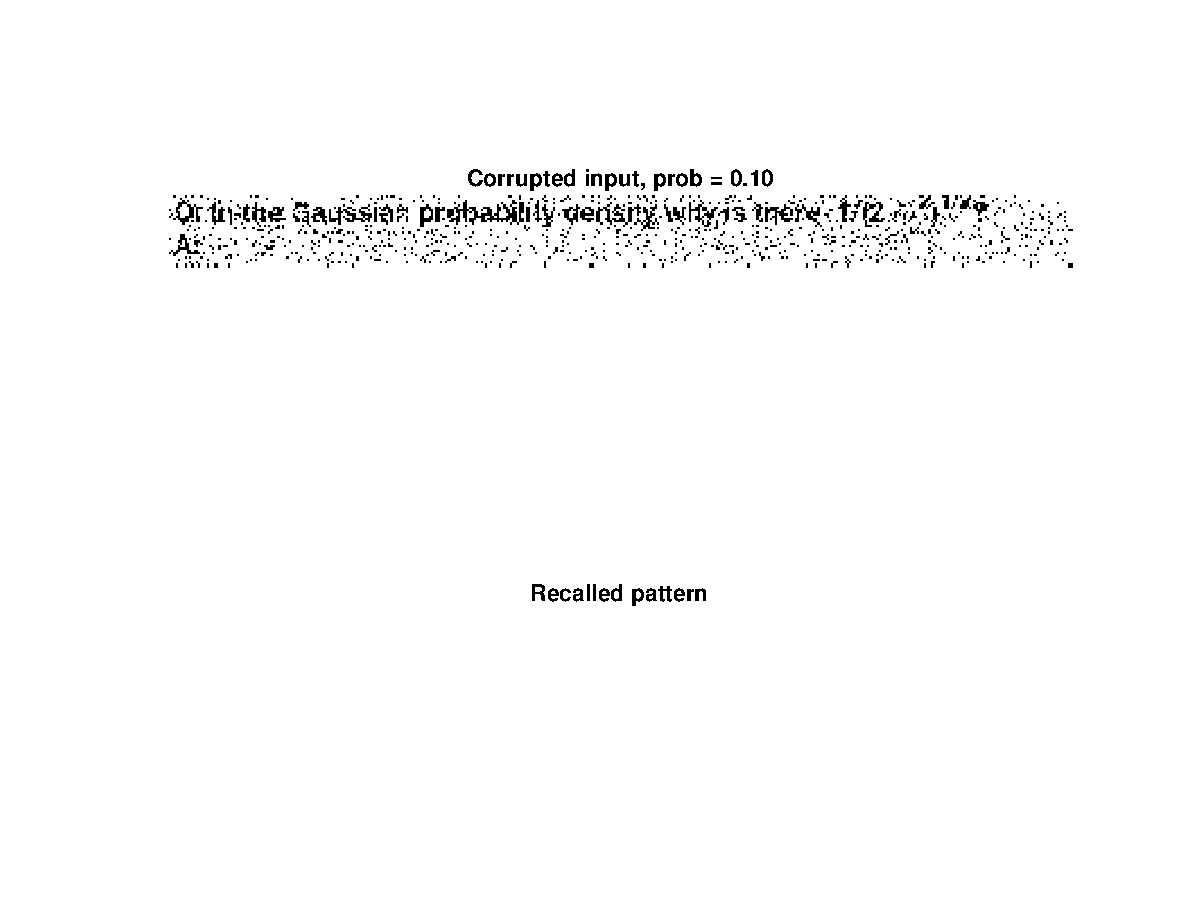
\includegraphics[width=1\textwidth]{q7corrupt.eps}
  \caption{The dynamics for question 7 at different levels of corruption.}
  \label{fig:q7corrupt}
  \end{figure}
\end{document}
